\chapter{Methodology}\label{chapter:Methodology}
The following chapter explains how the first four steps of the plan are used in the forecasting task for this Interdisciplinary Project in detail. Step five, the results and evaluation, is discussed in the next chapters.\newline
First of all the specific problem will be defined properly. Next the information needed will be specified and gathered. This data is processed in the preliminary analysis and fitted to models.
\section{Problem Definition}\label{section:Problem Definition}
According to the process some general questions have to be solved before the forecast is started. For this purpose a stakeholder analysis is done and a SIPOC diagram is created (Tabular \ref{tab:sipoc}).

\begin{table}[h]
\centering
\caption{SIPOC Diagram derived from the five basic steps}
\label{tab:sipoc}
\scalebox{0.75}{%
\begin{tabular}{|l|l|l|l|l|}
\hline
Supplier                                                                                    & Input                                       & Process                                                          & Output                                 & Customer                                            \\ \hline
\begin{tabular}[c]{@{}l@{}}Emanuel Pallua (COO)\\ Sebastian Sondheimer (BI)\\ Stefan Rothlehner(CTO)\\ Sergej Krauze (CTO)\\ Operations Team\end{tabular} & \begin{tabular}[c]{@{}l@{}}Knowledge\\ Experience\\ Historic Database\end{tabular} & \begin{tabular}[c]{@{}l@{}}Preliminary Analysis\\ Choosing Models\\ Fitting Models\\ Forecasting\\ Evaluating\end{tabular} & \begin{tabular}[c]{@{}l@{}}Forecast\\ Evaluation\\ Result\end{tabular} & \begin{tabular}[c]{@{}l@{}}Emanuel Pallua\\ Sebastian Sondheimer\\ Operation Team\end{tabular} \\ \hline
\end{tabular}}
\end{table}
Emanuel Pallua is identified as the first stakeholder. He is Chief of Operations at VOLO and the one who requested the forecast. Setting boundaries and demanding his needs makes him source and customer according to the SIPOC diagram. His goal of this forecast is to decrease "waste". Waste is defined as idle times for drivers, like being at the restaurant too early or food losing freshness by lying at the restaurant for too long. Another goal is to save money by maximizing the utilization of drivers and thus decreasing the fleet size. In general he wants a robust forecasting process which can be continuously improved and automated in the future for daily usage. \newline
The second source and customer in one person is Sebastian Sondheimer who is with Business Intelligence. His aim is to optimize the whole process of VOLO, the same as for Emanuel Pallua. He supports the forecast process by adding his knowledge of the current key numbers of VOLO. He suggests using only a few performance factors for the forecast, namely current slot (lunch, afternoon or dinner), current day, weekday, the week before and the weekday in the last month.\newline
On technical side there Stefan Rothlehner and Sergej Krauze, both Chief Technical Officers, as sources. Stefan Rothlehner is responsible for the backend and delivers the data. The information of the orders is extracted from the PostgreSQl database which is hosted on heroku. Sergej Krauze who is responsible for the Traveling Salesman Algorithm has the requirement that the language the forecast should be written in is Java. Since his work is already in Java and the forecast, once decided that it should be integrated, could be integrated without much additional effort.\newline
The last source and customer is the Operations Team since they are involved in the everyday business. They support the algorithm with their real life scenario knowledge. Their experience is that a 15 minute estimation works reasonably well. In their opinion a decrease of 50\% waste would make it worth to implement the algorithm. In order to have a benchmark for the results of the forecast, the error of their current assumptions will be calculated.
\newline\newline\textbf{Problem Statement}\newline
The goal is to research a forecast for preparation times of meals. The approach should be simple and easy to implement with the Traveling Salesman Algorithm. Reduction of waste should be significant over the current approach.
\section{Gathering Information}\label{section:Gathering Information}
The data for the forecast is taken from the PostgreSQL database of the backend. Every order from the beginning of VOLO in September has been processed and stored in this database. Each order has a timestamps for each step of the delivery process. This way a rich set of historical data has piled up and is available. For the forecast two data samples are downloaded at different points in time, one to create the forecast, the training data set, and another one to compare the results to, the test data set. They were dumped on the 26th of March and the 29th of April and contained 3034 and 4973 orders. The downloaded data sets were saved in comma separated values files, short csv files.\newline
This raw data has some weaknesses. The biggest one is the size of the gathered data. Forecasts need big amounts of information to generate a meaningful result. Since some restaurants have too few orders or a lot of bad data for the preparation times, additional expertise has to be put into the forecast. This expertise was taken from the Operation Team. They have to deal with orders on a daily basis and right now have to "forecast" the point in time the driver has to be at the restaurant on their own. In their experience an estimation of around 15 minutes is a more or less accurate guess for most restaurants except for some which are known for their unpredictability.\newline
In order to use the datasets from the csv files, it has to be parsed into objects in the Java program. For this purpose a csv parser library is used. The library reads the csv file and matches the orders from the database to the OrderModel.class of the code. Not all attributes of the database are used, only the one related to the forecast are picked from the information. Since there is no tracking in the restaurant for the preparation time, it was decided to take the time interval from the point in time at which the restaurant knows from the order until the driver leaves the restaurant. In the process of volo, the printer in the restaurant prints the recipe at the same time the driver accepts the delivery, which is saved in the database as \texttt{accepted\_at}. The timestamp of the driver leaving the restaurant is saved in \texttt{delivery\_started\_at}. Since it is not the task to figure out the exact the preparation time but the time from when the order is send to the restaurant and when the driver can pick it up, no modification to the time are done.
\section{Preliminary Analysis}\label{section:Preliminary Analysis}
There are many factors which can influence the preparation times of the restaurant. Some are of external nature, some internal nature. The weather or season can have an effect on how busy the restaurant is which can cause different cooking times or when a cook is ill the restaurant can be overwhelmed by too many orders.\newline
There are also other factors, like marketing campaigns, which can influence the results, but this has not happened in the recorded time frame.\newline
In order to discover these patterns and get a feeling for the data the preliminary analysis is done.
\subsection{Raw Data Cleanup}\label{subsection:Raw Data Cleanup}
First of all the data has be cleaned and a rough overview for the dimensions of the data should be generated. This is done to get a feeling of the time frame a restaurant usually needs to prepare an order. This provides an estimation of what to expect and clue whether the result of a forecast is totally unrealistic or pretty close to what is possible. In addition to the average time analysis a visualization of the data is done as well. This is done in a time series plot on which it is very easy to see anomalies or patterns of the raw data.\newline

\begin{figure}[h]
\begin{center}
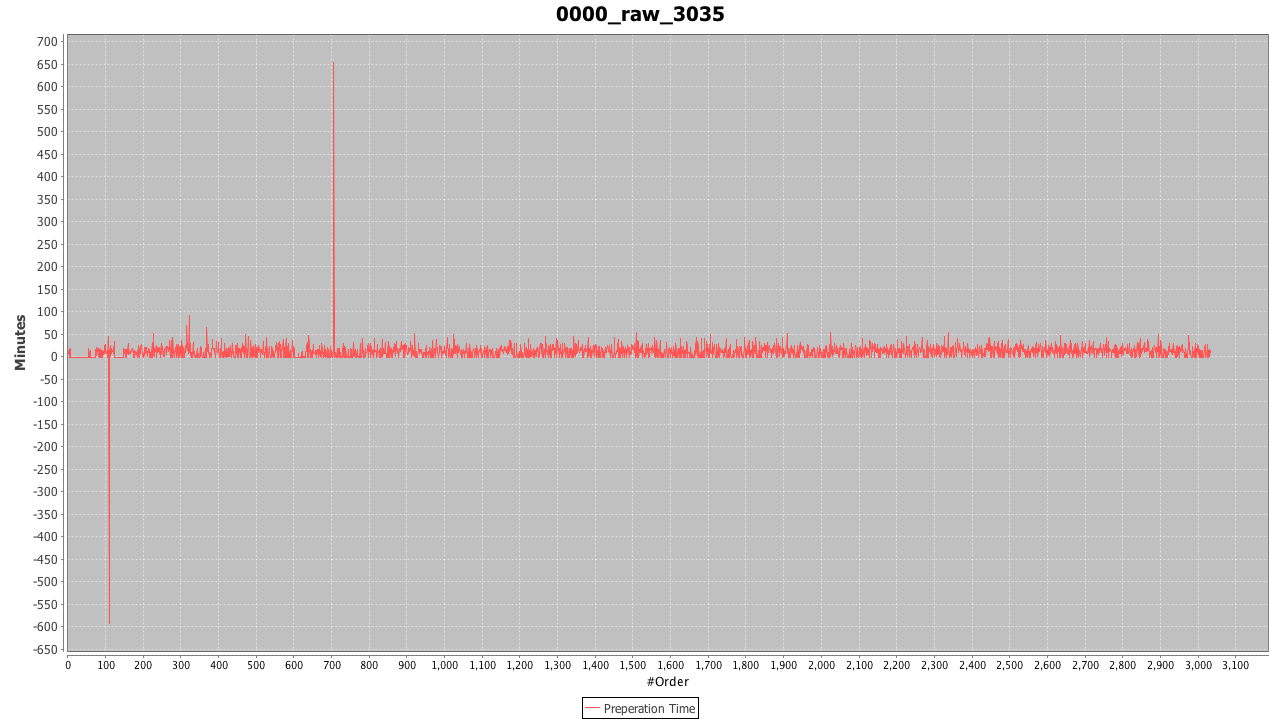
\includegraphics[width=10cm]{images/0000_raw_3035.png}
\caption{Observations of preparation time of all orders without any data clean up}
\label{fig:0000_raw_3035}
\end{center}
\end{figure}

As the first step of the raw data cleanup, the training data is put into a time series graph (Fig. \ref{fig:0000_raw_3035}). This analysis reveals problems the data has. The training data set still contains unfinished orders, bugged order, which were finished at a wrong point of time, and orders which have corrupted timestamps. These three types of unusable orders receive a total time of "-1" since either their \texttt{accepted\_at} timestamp is missing or not readable. In case that the orders \texttt{delivery\_started\_at} timestamp is before the \texttt{accepted\_at} timestamp a negative value is visible. This events can be observed in many cases in the time series graph and result in an average preparation time of 12 minutes. In order to get realistic results these flaws in the data set have to be removed. This is done by ignoring all values which are below 0 minutes in the forecast. This action increases the average preparation time to 16 minutes which is much higher than the first result but free of wrong values. The data set is visualised in Figure \ref{fig:0000_invalid_2204} which, in contrast to Figure \ref{fig:0000_raw_3035}, does not contain any negative values.

\begin{figure}[h]
\begin{center}
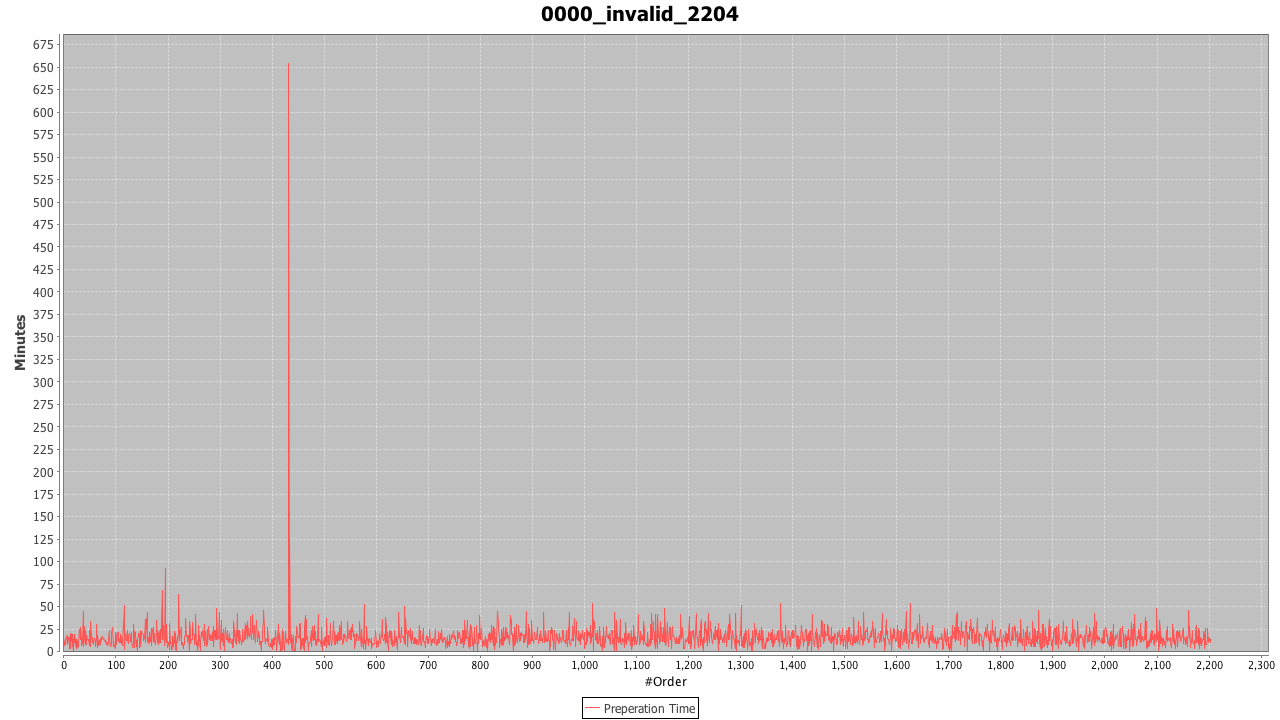
\includegraphics[width=10cm]{images/0000_invalid_2204.png}
\caption{Observations of preparation time of all orders without invalid values}
\label{fig:0000_invalid_2204}
\end{center}
\end{figure}

After removing the obviously unusable orders the data looks a lot more usable. The only problem are the orders which were finished long after they have been started. It can be assumed that these times were either caused by bugged software or human error in the process and remove them from the data set. For this purpose the Grubbs training for outliers is applied to the dataset and all values that seem not to come from a normally distributed population are removed (\cite{Grubbs}). Figure \ref{fig:0000_grubbed_2201} shows how this action influences the graph. This results in an average preparation time of 15 minutes which is the same result as the operations team suggest to use as a basis.

\begin{figure}[h]
\begin{center}
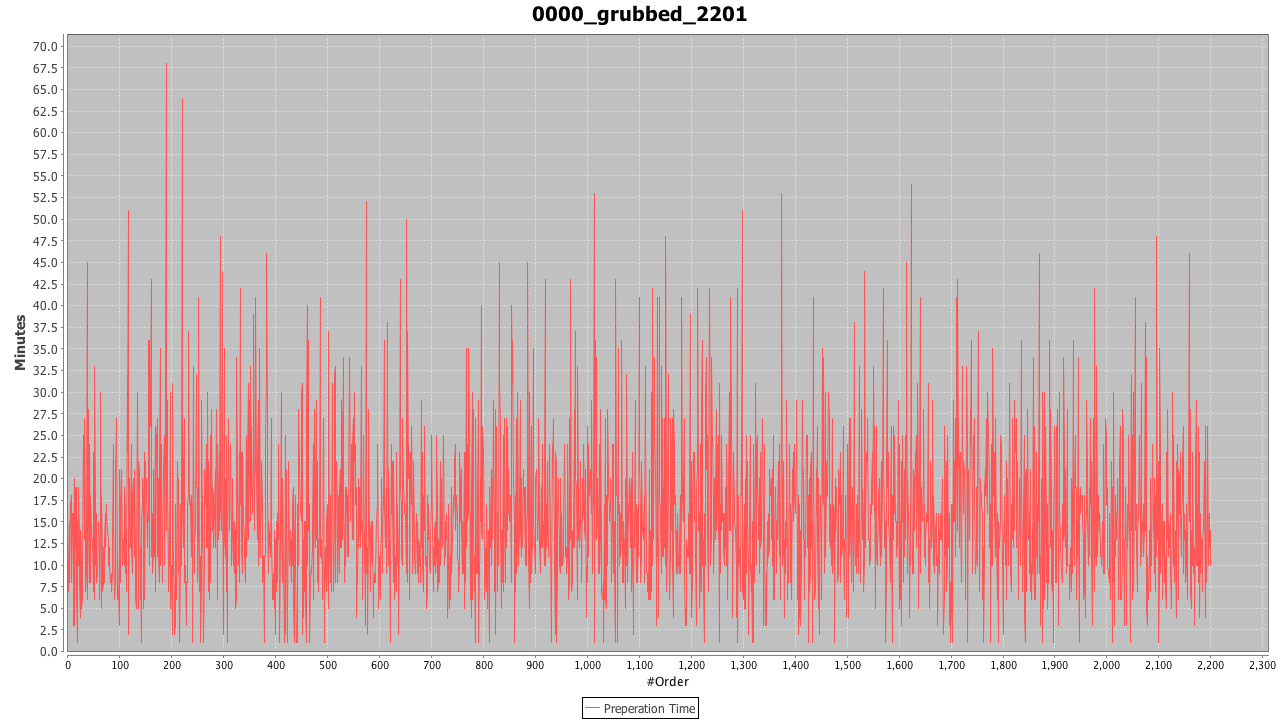
\includegraphics[width=10cm]{images/0000_grubbed_2201.png}
\caption{Observations of preparation time of all orders without invalid values and outliers}
\label{fig:0000_grubbed_2201}
\end{center}
\end{figure}



Now the usable training dataset is extracted from the input data, it can be analyzed for patterns, trends or similarities. For this purpose a time component has to be introduced into the graph since putting order after order does not include it. That is why orders are summed up by day and visualized by average preparation time per day in Figure \ref{fig:0000_byDay_97}. The only usable information that can be extracted is that the average preparation time varies from day to day.

\begin{figure}[h]
\begin{center}
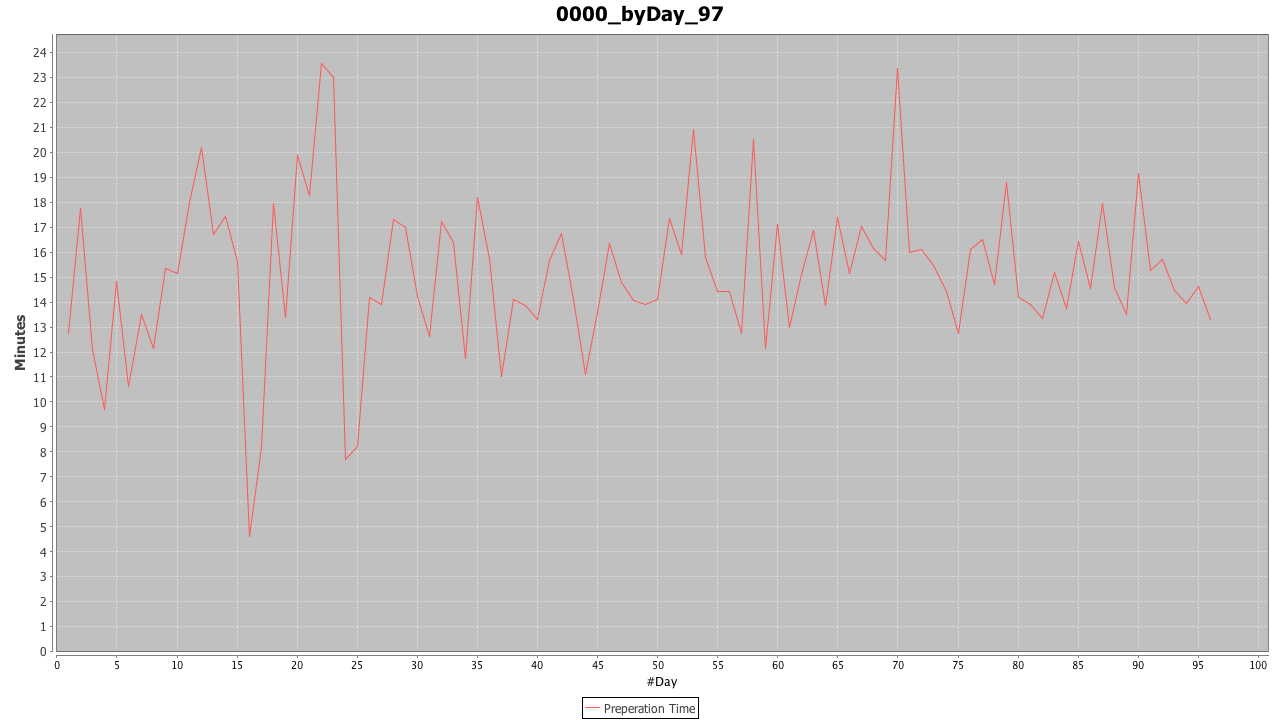
\includegraphics[width=10cm]{images/0000_byDay_97.png}
\caption{Average preparation time per day}
\label{fig:0000_byDay_97}
\end{center}
\end{figure}

Since no clear trend or pattern can be observed in a day by day analysis (Figure \ref{fig:0000_byDay_97}), a box and whisker diagram is created from the data (Figure \ref{fig:triple_boxWhisker}). It shows the median and average preparation time as line and point inside the box. The box represents the upper and lower quartile of preparation times in which 50 \% of the data is while the red whiskers visualize the area without outliers, which are red circles and a red triangle in case they are out of scale. The purpose of this graph is to give an overview of the set of values of the preparation time and the boundaries most of the orders are located in. The data was divided into different categories.\newline
The first diagram in Figure \ref{fig:triple_boxWhisker} on the left is on week basis. It was created to see if there is a trend over time as the company expertise grows. The only observation is that can be made is that after fluctuating preparation times in the first weeks it gets more constant towards the end.\newline
Since no conclusion can be drawn from this categorization, a box whisker diagram for each slot was created (Figure \ref{fig:triple_boxWhisker}, middle). The day is divided into three slots, the big meals, lunch and dinner, as well as the time between these, the afternoon, which should be not as busy as the meal times. The diagram shows no real difference in preparation times between the slots so this has to be inspected in a different categorization containing slots.\newline
This is done by visualizing the slots for each weekday in order to identify special behaviour since weekdays can have strong differences in terms of load for the restaurant (Figure \ref{fig:triple_boxWhisker}, right). This is done since it contains two different key information. Slots and weekdays alone do not have as much information as the two combined. For example on a sunday evening many people like to go to a restaurant and do not order while in the week offices sometimes order big deliveries for lunch. The values in the diagram do not vary that much which can be due to a low training dataset. It could also be separated between weekend and weekdays but there is not enough data to do this and gain additional information.\newline
The difference between slots on weekdays as well as between weekdays is more significant than all other diagrams before and should be considered when creating the model.

\begin{figure}[htp]

\centering
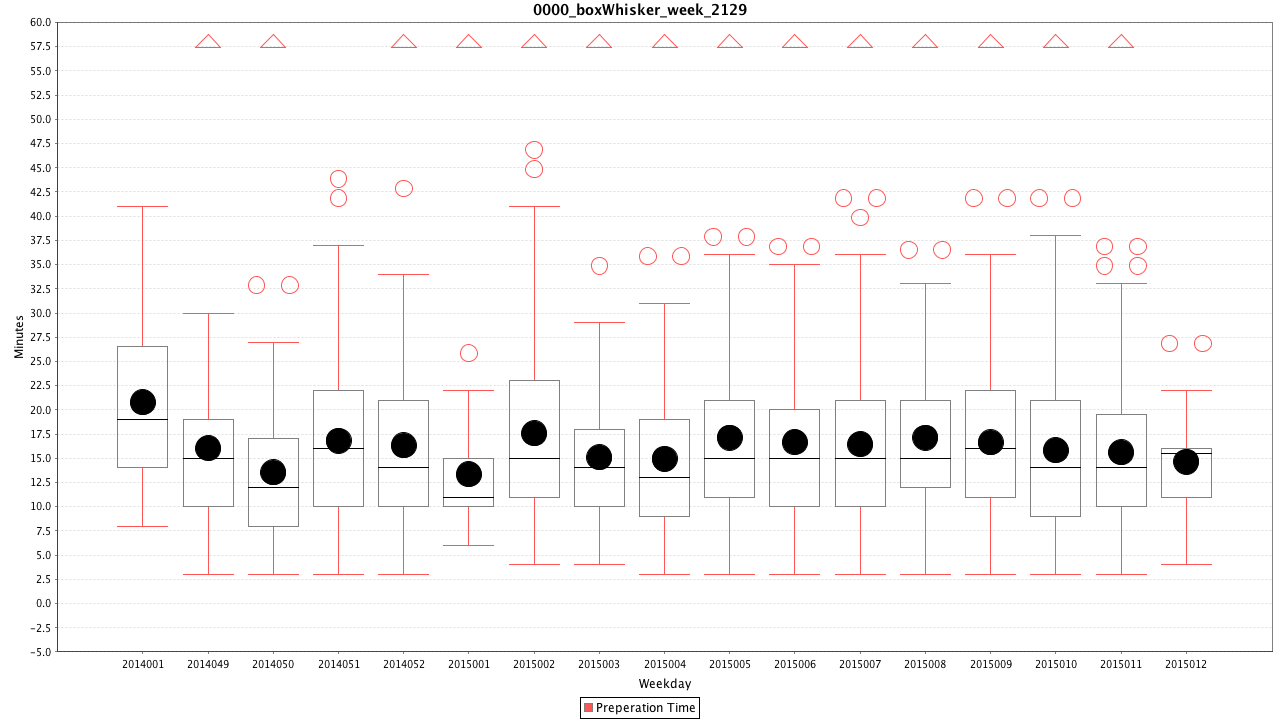
\includegraphics[width=.3\textwidth]{images/0000_boxWhisker_week_2129.png}\hfill
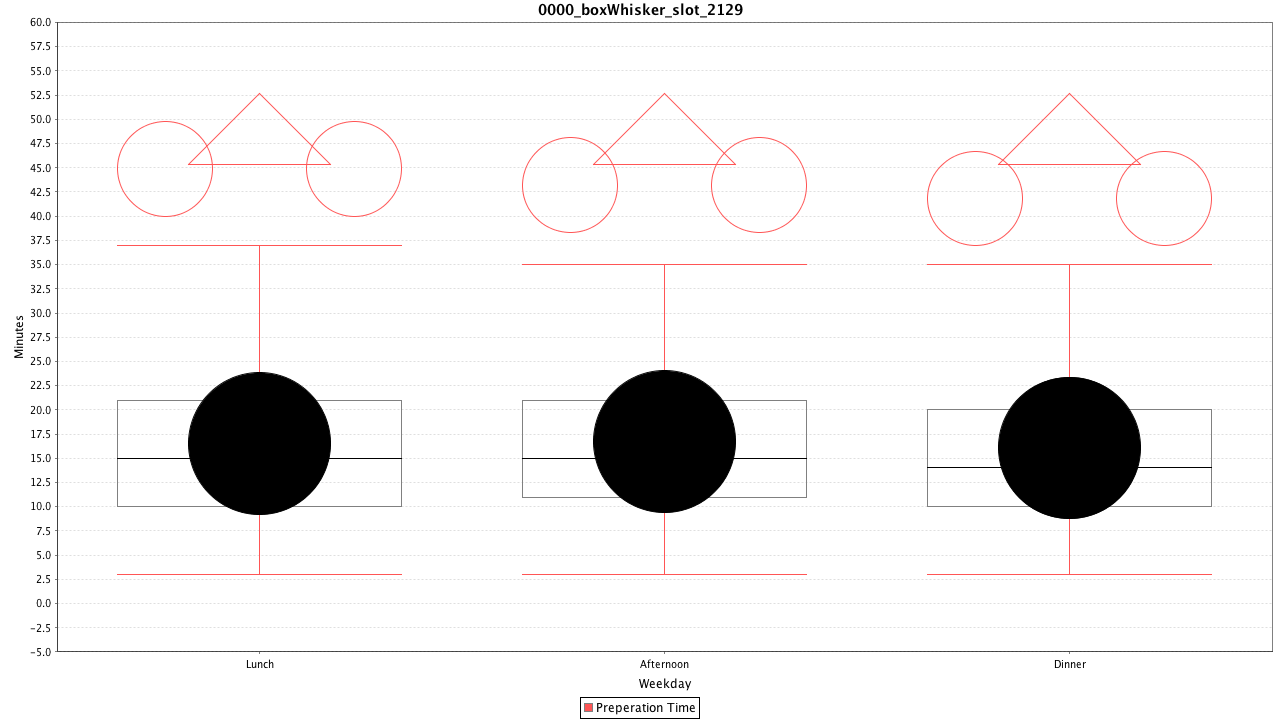
\includegraphics[width=.3\textwidth]{images/0000_boxWhisker_slot_2129.png}\hfill
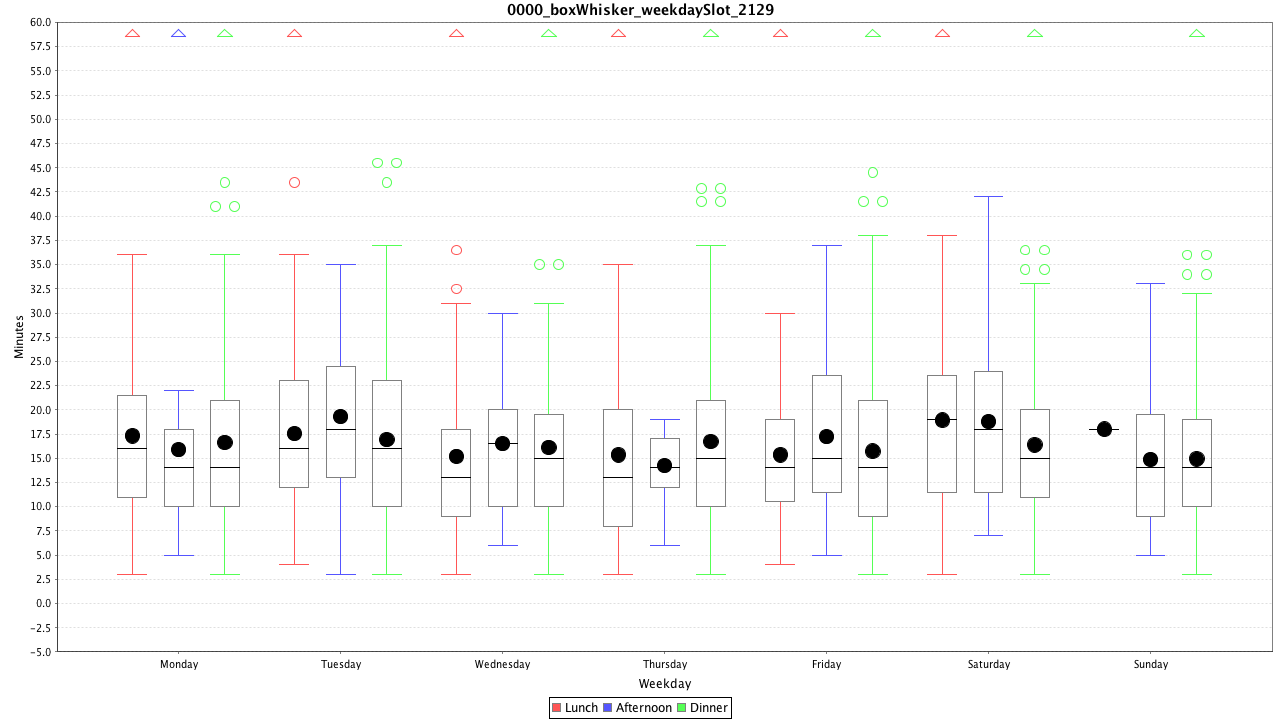
\includegraphics[width=.3\textwidth]{images/0000_boxWhisker_weekdaySlot_2129.png}

\caption{Box-Whisker diagrams with different time categorization. By Week (left), by Slot (middle) and by Weekday-Slot (right).}
\label{fig:triple_boxWhisker}

\end{figure}

All these lessons learned from the clean up of the data is also applied to the test data set which is used later.

\subsection{Restaurant Wise Proceeding}\label{subsection:Restaurant Wise Proceeding}
The restaurants preparation times can be very different. There are restaurants, which have already pre-cooked ingredients, others who have a very simple way of preparing the meal, like sandwiches, and others are crowded at a certain time and will take longer, preparation times are very different. A pizzeria has other preparation times than a burrito take away.\newline
This suggest distinguishing by restaurant. Initially two categories are created, one restaurant agnostic and another one restaurant specific. For the evaluation of the restaurant specific forecast yum2take is chosen. It is the most mature customer of VOLO.\newline
In order to get a first look at the restaurant specific data, a diagram with slot and weekday differentiation is created in Figure \ref{fig:1_boxWhisker_weekdaySlot_686}.
\begin{figure}[h]
\begin{center}
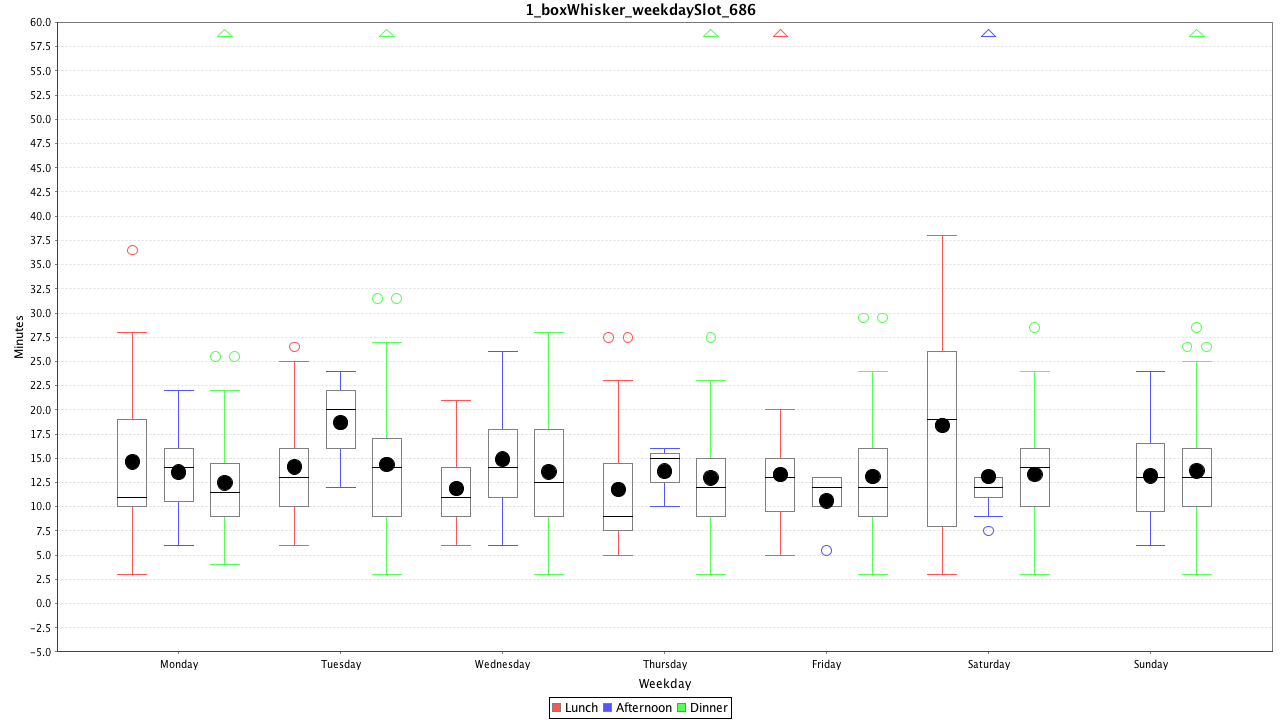
\includegraphics[width=10cm]{images/1_boxWhisker_weekdaySlot_686.png}
\caption{Observations of preparation time of all orders at yum2take without invalid values and outliers}
\label{fig:1_boxWhisker_weekdaySlot_686}
\end{center}
\end{figure}
The distribution in the diagram for yum2take is clearly different from the overall visualization. This consolidates the assumption that restaurants should be looked at separately. The average times are also different. For the raw data 10.2 minutes are the average, when cleaning the data from invalid values it increased to 13.5 minutes and without the outliers it lowered to 13.1 minutes.
\subsection{Current Assumption}
The RMSE of the current forecasting mechanism where every preparation time is supposed to be 15 minutes is calculated from the training data is 8.5 minutes.
\section{Choosing and Fitting Models}\label{Choosing and Fitting Models}
After the preliminary analysis it is time to fit the data to models for the forecast. A model combines three dimensions, the algorithm, the restaurant category and a time category.
\subsection{Time Categorizing of Orders}\label{subsection:Categorizing by Order}
When categorized by time, only orders in a specific time window are used to calculate the forecast value for the current order. The time window is always relative to the current order. The following time categories were chosen:\newline
\newline\textbf{No Time Categorization}\newline
No time categorization means that for the forecast of the current order all predecessing orders are taken into account. This is done in order to treat all orders the same and get a simple forecast.
\newline\textbf{Day Categorization}\newline
When using day categorization, only the orders before the current one on the same day are used to calculate the forecast value. The day categorization is done since from one day to another day different conditions in the restaurant can change, e.g. staff is ill, which has an impact on that day.
\newline\textbf{Week Categorization}\newline
The week categorization is done to take larger events in account when forecasting. Examples could be marketing campaigns. In order to consider such events, this categorization uses all predecessing orders of the calendar week for the calculation.
\newline\textbf{Weekday Categorization}\newline
Weekdays are also different from each other and have to be considered since they cause different utilization of restaurants, e.g. on sundays markets are closed and people tend to order. For this categorization all orders before the current on this weekday are used for the forecast of the order.
\newline\textbf{Single Minislot Categorization}\newline
The minislot categorization divides the day into half hour slots. For each forecast for an order the orders before the current one in this slot are used. This is done to consider short time fluctuations caused by peak times, e.g. the half hour in which most people do their lunch or shortly before eight in the evening before the prime time movie starts.
\newline\textbf{Slot Categorization}\newline
In the requirements three main phases, the slot, were declared. These slots are lunch, dinner and the time in between and they cause different traffic for the restaurants, lunch and dinner being high traffic while the time in between is not so crowded. In order to consider these day specific differences, it can be applied together with the other categorizations, except minislot, to improve the accuracy of the forecast. For example when using day and slot categorization, not all predecessing orders of the current day are considered for the forecast but only the ones in the slot before the current order.

\newline
Before the actual forecast can be done, the edge case of not having predecessing orders for the current order, has to be resolved. Since the operations teams suggested a 15 minute basic time for preparation, this time is always taken when no forecast value can be generated for the current order.
\subsection{Combination of Time Categorizations}\label{subsection:Categorizing by Order}
These categorizations can be combines to create a more complex forecasting model. This model is created by using an algorithm, the restaurant category and multiple time categories. It is calculated with different weightings of the time categories, which is done in 5\% steps, e.g. 5\% category A, 20\% category B and 75\% category C. This is done for all possible combinations. In order to get a meaningful forecast, the most important time categories are chosen for the model. There are three categories with two subcategories. One is current slot and current day, since this categories contain information about the current load in the restaurant. Another one is the current slot in the last 7 days and the whole last 7 days. This categories can give information about small trends, like marketing campaigns. The last category is the current slot of the weekday over the last 4 weeks and the weekday itself over the last 4 weeks, which can supply information about general patterns, like sunday is always a crowded day.\newline
This combination is done to consider the behavior of orders depending on their point in time.
